% !TeX spellcheck = en_US
\documentclass[10pt]{beamer}
\usepackage[latin1]{inputenc}
\usetheme{Warsaw}
\usecolortheme{beaver}
%\usepackage{braket}
\usepackage{amsmath}
\usepackage{amsfonts}
\usepackage{amssymb}
\usepackage{graphicx}
%\setbeamerfont{page number in head/foot}{size=\normalsize}
%\setbeamertemplate{footline}[frame number]
\usepackage{ifthen}
\usepackage{animate}
\newcommand*\oldmacro{}%
\let\oldmacro\insertshorttitle%
\renewcommand*\insertshorttitle{%
	\oldmacro\hfill%
	\insertframenumber\,/\,\inserttotalframenumber}
\setbeamercovered{transparent}
\usepackage{tikz}
\usetikzlibrary{calc}
\usepackage{pgfplots}
\usepackage{tikz-3dplot}
\usetikzlibrary{decorations.markings}
\usetikzlibrary{shapes,arrows}
\newcommand{\midarrowright}{\tikz \draw[-triangle 90] (0,0) -- +(.1,0);}
\newcommand{\midarrowup}{\tikz \draw[-triangle 90] (0,0) -- +(0,.1);}

\usetikzlibrary{shadings, calc, decorations.markings}
\tikzset{->-/.style={decoration={
			markings,
			mark=at position #1 with {\arrow{<}}},postaction={decorate}},
	->-/.default=0.3,
}

\tikzset{->>-/.style={decoration={
			markings,
			mark=at position #1 with {\arrow{<}}},postaction={decorate}},
	->>-/.default=0.7,
}

\newcommand\ds{\displaystyle}
\newcommand\ts{\textstyle}
\newcommand{\mb}{\mathbf}
%\renewcommand{\thenotation}{}
%\renewcommand{\theequation}{\thesection.\arabic{equation}}
\def\Caption #1{\caption{\footnotesize #1}}
%\renewcommand\Caption{#1}{\Caption{\small{#1}}}
%\def\Caption #1{\Caption{\small{{#1}}}}

\def \Bfemph #1{\textbf{\emph{#1}}}


%\def\Proof.{{\medbreak\noindent{\it Dimostrazione}\enspace}}
\def\Proof{{\medbreak\noindent{\textbf{Proof.} }}}
\def\Proofsketch{{\medbreak\noindent{\textbf{Sketch of proof.} }}}
\def\endproof{~\hfill $\blacksquare$}
%\def\endproof{\hfill$\square$\par\medskip}

\def\Svolgimento{{\medbreak\noindent{\textit{Execution.} }}}
\def\Suggerimento{{\medbreak\noindent{\textit{Hint:} }}}


\def\mR{{\mathbb R}}
\def\mC{{\mathbb C}}
\newcommand{\parz}[2]{ \frac{\partial #1}{\partial #2}}
\newcommand{\deri}[2]{\displaystyle \frac{\dd #1}{\dd #2}}
\renewcommand{\Re}{\text{Re }}
\renewcommand{\Im}{\text{Im }}
%\renewcommand{\theta}{\vartheta}
\newcommand{\Int}{\text{Int }}
\newcommand{\Ext}{\text{Ext }}
\newcommand{\supp}{\text{supp}}
\newcommand{\mD}{\mathcal{D}}
\newcommand{\dd}{\mathrm d}
\newcommand{\norm}[1]{\displaystyle \left \| #1 \right \|}
\renewcommand{\div}{\operatorname{div}}
\newcommand{\rot}{\operatorname{rot}}
\newcommand{\grad}{\operatorname{grad}}
\newcommand{\id}{\mathds{1}}
\newcommand{\mM}{\mathrm{M}}
\newcommand{\mT}{\mathrm{T}}
%\renewcommand{\to}{\longrightarrow}
\newcommand{\scalar}[2]{\left\langle #1, #2 \right\rangle}
\newcommand{\mf}[1]{\mathbf{#1}}

\def\Xint#1{\mathchoice 
	{\XXint\displaystyle\textstyle{#1}}% 
	{\XXint\textstyle\scriptstyle{#1}}% 
	{\XXint\scriptstyle\scriptscriptstyle{#1}}% 
	{\XXint\scriptscriptstyle\scriptscriptstyle{#1}}% 
	\!\int} 
\def\XXint#1#2#3{{\setbox0=\hbox{$#1{#2#3}{\int}$} 
		\vcenter{\hbox{$#2#3$}}\kern-.5\wd0}} 
\def\Mint{\Xint -}


\renewcommand{\hat}[1]{\widehat{#1}}
\renewcommand{\theta}{\vartheta}
\renewcommand{\epsilon}{\varepsilon}
%\renewcommand{\phi}{\varphi}
\newcommand{\res}{\mathop{\mathrm{Res }}}

\newcommand{\colonna}[2]{\begin{pmatrix}
		#1 \\ #2
\end{pmatrix}}
\newcommand{\riga}[2]{\begin{pmatrix}
		#1 & #2
\end{pmatrix}}
%%%%%%%%%%%%%%%%%%%%%%%%%%%%%%%%%%%%%%%%%%%%%%%%%%%%%%%%%%%%%%%%%%%%%%%%%%%%%%%%%%%%%%%%%%%

\newcounter{angle}
\setcounter{angle}{0}

\title{Soluzioni fondamentali per equazioni di tipo onda su variet� curve}
\author{Rubens Longhi}
\date


\begin{document}
	
	
	\begin{frame}
	 \maketitle
	 	 	\begin{center}
	 	\[\Box u=\delta\]
	 %\begin{columns}
	 	
	% \begin{column}{.48\linewidth}
	 %	Relatore: \textbf{Claudio Dappiaggi}
	% \end{column}
 % \begin{column}{.48\linewidth}
 %	Co-relatore: \textbf{Nicol� Drago}
 %\end{column}
	% \end{columns}
 
 

	 	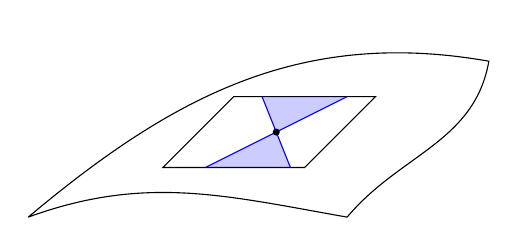
\begin{tikzpicture}[scale=0.9]
	 	\tikzstyle{every node}=[font=\scriptsize]
	 	
	 	\draw (1,2.8) to[out=40,in=170] (7.5,5) %node at (7,4.8) {$\mathrm{M}$}
	 	to[out=-100,in=50]  (5.5,2.8) to[out=170,in=20] (1,2.8);
	 	
	 	\begin{scope}[shift={(0.5,0)},scale=1]
	 	\clip (2.2,3.4)-- (4.7,3.4) -- (5.7,4.6) -- (3.2,4.6) -- cycle;
	 	\draw [draw=black, thin, fill=white] (2.4,3.5)-- (4.4,3.5) -- (5.4,4.5) -- (3.4,4.5) -- cycle;
	 	%\draw [ultra thin, dashed] (1,2.8) to[out=40,in=170] (7.5,5) %node at (7,4.8) {$\mathrm{M}$}
	 	% to[out=-100,in=50]  (5.5,2.8) to[out=170,in=20] (1,2.8);
	 	
	 	\draw [thin, color=blue, fill=blue, fill opacity=0.2] (3,3.5) -- (4,4) -- (4.2,3.5) ;
	 	
	 	\draw [thin, color=blue, fill=blue, fill opacity=0.2] (3.8,4.5) -- (4,4) -- (5,4.5);
	 	
	 	%\draw [thin, color=blue, fill=blue, fill opacity=0.2] (3,3.5) -- (5,4.5)-- (3.8,4.5) -- (4.2,3.5) -- (3.8,4.5);
	 	\fill [black] (4,4) circle (0.05cm) %node [left] {$x$}
	 	;
	 	\end{scope}
	 	
	 	%\node at (5.3,4) {$\mathrm{T}_x\mathrm{M}$};
	 	
	 	\end{tikzpicture}
	\end{center}
	\begin{center}
		
	\end{center}

	\end{frame}
	
	\begin{frame}
		\frametitle{Equazioni di tipo ondulatorio}
		%\framesubtitle{Un preambolo}
\tikzstyle{na} = [baseline=-.5ex]

Gli operatori di tipo ondulatorio governano la dinamica di molti sistemi fisici
\begin{itemize}
	\item<+-| alert@+> Operatore d'onda: il d'Alembertiano\\

	$$\displaystyle \Box=\frac{\partial^2}{\partial t^2}-\sum_{j=1}^{n}\frac{\partial^2}{\partial x_j^2}$$
	\item<+-| alert@+> Equazioni di Maxwell
\begin{equation*}
\begin{cases}
\Box A^\mu-\partial^\mu\partial_\nu A^\nu=4\pi J^\mu\\
\partial_\mu J^\mu=0
\end{cases}
\end{equation*}
	\item<+-| alert@+> Equazione di Klein-Gordon
	\begin{equation*}
	(\Box +m^2)\psi=f
	\end{equation*}
\end{itemize}




\end{frame}


\begin{frame}
	\frametitle{Le soluzioni fondamentali}
	\framesubtitle{Un metodo costruttivo}
	
	\begin{itemize}
		\item<+-| alert@+> Vogliamo risolvere in $\mR^N$ una qualsiasi equazione differenziale scalare non omogenea \[	P\psi=f		\] nell'incognita $\psi$ con sorgente $f$.\bigskip
		\item<+-| alert@+> Le soluzioni saranno date da $$\psi=\psi_0+\psi_f$$ dove $\psi_0$ risolve l'omogenea associata e $\psi_f$ � una soluzione particolare
	\end{itemize}
	
	
	%Vogliamo risolvere su una variet� $\mM$ una qualsiasi equazione differenziale non omogenea \[	Pf=\psi		\] nell'incognita $f$ con generica sorgente $\psi$.\\ \pause
	%\bigskip
	%La studiamo nel caso di una sorgente elementare deltiforme nel punto $x$ \[	Pu_x=\delta_x		\]
	%e cerchiamo soluzioni distribuzionali $u_x\in\mD'(\mM)$.\\	\pause
	%\bigskip		
	%Troviamo una soluzione a $Pf=\psi$ integrando opportunamente la soluzione fondamentale su tutti i punti $x\in\supp\,\psi$.

	
	
	
	
	
\end{frame}

\begin{frame}
	\frametitle{Le soluzioni fondamentali}
	\framesubtitle{Un metodo costruttivo}
	\begin{itemize}
		\item<+-| alert@+> Risolviamo per un punto $x\in\mR^N$  \[	Pu_x=\delta_x		\]
		con $u_x\in\mD'(\mR^N)$. $u_x$ � detta \textcolor{red}{\textbf{soluzione fondamentale}} per $P$ in $x$
		\bigskip
		\item<+-| alert@+> Troviamo una soluzione particolare tramite la \textcolor{red}{\textbf{convoluzione}}
		\[	\psi_f=u_x*f		\]
		\item<+-| alert@+> Nel caso di operatori d'onda, otteniamo una soluzione per l'omogenea dalla differenza di due soluzioni fondamentali
	\end{itemize}
\end{frame}


\begin{frame}
	
	\frametitle{L'operatore d'onda in Minkowski}
	\framesubtitle{Il caso dello spaziotempo piatto}
	\begin{block}{Equazione di Klein-Gordon con massa nulla}
		\centering $\Box\psi=f$
	\end{block}
		\begin{block}
			
		Spaziotempo piatto di Minkowski $\mathbb{M}^n$ $\rightarrow$ $1$ dimensione temporale e $n$ dimensioni spaziali\pause
	\end{block}\bigskip
	
	
	L'invarianza traslazionale ci consente di limitare il problema per $\Box$ all'origine: $$ \Box u_0=\delta_0$$ e di utilizzare la tecnica della trasformata di Fourier.\\

	
	
	
	
\end{frame}

\begin{frame}
	\frametitle{La tecnica della trasformata di Fourier}
	La PDE in $(t,\mf{x})$ diventa l'equazione algebrica nello spazio delle fasi $(\omega,\mf{k})$
	\[	(|\mf{k}|^2-\omega^2)\widehat{u}=1	\]\pause
\begin{block}
	
	Troviamo due soluzioni linearmente \textcolor{red}{\textbf{indipendenti}}, che danno luogo a due soluzioni fondamentali $G^+$ e $G^-$ dette \textcolor{red}{\textbf{ritardata}} e \textcolor{red}{\textbf{avanzata}}
\end{block}\bigskip
\begin{equation*}
G^\pm(x)=\frac{1}{(2\pi)^{n+1}}\lim_{\epsilon\to 0^+}\int_{\mR^{n+1}}\frac{e^{i\langle k,x\rangle}}{|\mathbf{k}|^2-(\omega\pm i\epsilon)^2}\,\dd k
\end{equation*}
	
\end{frame}


\begin{frame}
	\frametitle{Le soluzioni fondamentali ritardata e avanzata}
	\begin{columns}
		\begin{column}{.48\linewidth}
			\begin{block}{\centering La soluzione ritardata}
				
				$\supp\,G^+$ � nel \textcolor{red}{\textbf{futuro causale}}
				\centering
				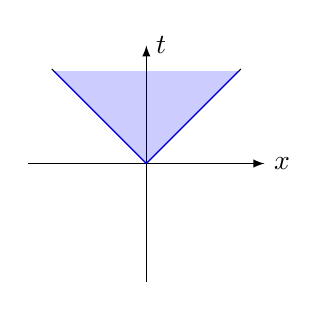
\begin{tikzpicture}[scale=0.3][>=latex]
				\coordinate (Origin)   at (0,0);
				\coordinate (XAxisMin) at (-5,0);
				\coordinate (XAxisMax) at (5,0);
				\coordinate (YAxisMin) at (0,-5);
				\coordinate (YAxisMax) at (0,5);
				\draw [thin,-latex] (XAxisMin) -- (XAxisMax) node[right] {$x$};% Draw x axis
				\draw [thin,-latex] (YAxisMin) -- (YAxisMax) node[right] {$t$};% Draw y axis
				
				%\clip (-5,-5) rectangle (10cm,10cm); % Clips the picture...
				
				\draw[thin] (0,0) -- (4,4);
				\draw[thin] (0,0) -- (-4,4);
				\begin{scope}
				\clip (-4,0) -- (4,0) -- (4,3.9)-- (-4,3.9) --cycle;
				\draw [thin, color=blue, fill=blue, fill opacity=0.2] (0,0) -- (4,4) -- (-4,4) --cycle ;
				\end{scope}
				%\node[fill=white,rounded corners=1pt,inner sep=0.5pt] at (0,2.5) {$G^+=\frac{1}{2}$};
				
				
				
				
				
				
				
				\end{tikzpicture}
			\end{block}
		\end{column}
		
		\begin{column}{.48\linewidth}
			\begin{block}{\centering La soluzione avanzata}
				
				$\supp\,G^-$ � nel \textcolor{red}{\textbf{passato causale}}
				\centering
				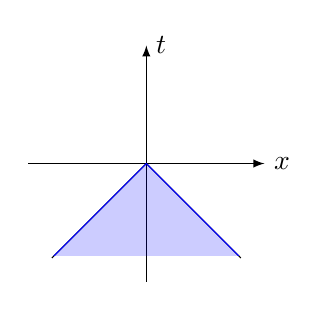
\begin{tikzpicture}[scale=0.3][>=latex]
				\coordinate (Origin)   at (0,0);
				\coordinate (XAxisMin) at (-5,0);
				\coordinate (XAxisMax) at (5,0);
				\coordinate (YAxisMin) at (0,-5);
				\coordinate (YAxisMax) at (0,5);
				\draw [thin,-latex] (XAxisMin) -- (XAxisMax) node[right] {$x$};% Draw x axis
				\draw [thin,-latex] (YAxisMin) -- (YAxisMax) node[right] {$t$};% Draw y axis
				
				%\clip (-5,-5) rectangle (10cm,10cm); % Clips the picture...
				
				
				\draw[thin] (0,0) -- (4,-4);
				\draw[thin] (0,0) -- (-4,-4);
				\begin{scope}
				\clip (-4,0) -- (4,0) -- (4,-3.9)-- (-4,-3.9) --cycle;
				\draw [thin, color=blue, fill=blue, fill opacity=0.2] (0,0) -- (4,-4) -- (-4,-4) --cycle ;
				\end{scope}
				%\node[fill=white,rounded corners=1pt,inner sep=0.5pt] at (0,-2.5) {$G^-=-\frac{1}{2}$};
				
				
				
				
				
				
				
				\end{tikzpicture}
			\end{block}
		\end{column}
	\end{columns}
	
\end{frame}





\begin{frame}
	\framesubtitle{Le soluzioni fondamentali in Minkowski}
	\frametitle{Il caso $n=1$ - onde su una corda}
 
	 
	\begin{columns}[t]
		\begin{column}{.48\linewidth}
		
			\begin{block}
				
				\begin{figure}
					\centering
					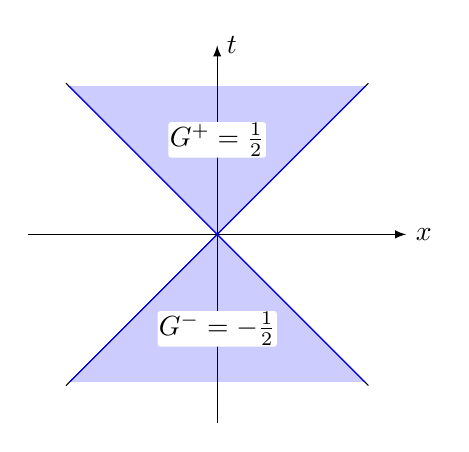
\begin{tikzpicture}[scale=0.48][>=latex]
						\coordinate (Origin)   at (0,0);
					\coordinate (XAxisMin) at (-5,0);
					\coordinate (XAxisMax) at (5,0);
					\coordinate (YAxisMin) at (0,-5);
					\coordinate (YAxisMax) at (0,5);
					\draw [thin,-latex] (XAxisMin) -- (XAxisMax) node[right] {$x$};% Draw x axis
					\draw [thin,-latex] (YAxisMin) -- (YAxisMax) node[right] {$t$};% Draw y axis
					
					%\clip (-5,-5) rectangle (10cm,10cm); % Clips the picture...
					
					\onslide<1>{\draw[thin] (0,0) -- (4,4);
						\draw[thin] (0,0) -- (-4,4);
						\begin{scope}
						\clip (-4,0) -- (4,0) -- (4,3.9)-- (-4,3.9) --cycle;
						\draw [thin, color=blue, fill=blue, fill opacity=0.2] (0,0) -- (4,4) -- (-4,4) --cycle ;
						\end{scope}
						\node[fill=white,rounded corners=1pt,inner sep=0.5pt] at (0,2.5) {$G^+=\frac{1}{2}$};
						
					}
				
					\onslide<2>{\draw[thin] (0,0) -- (4,-4);
						\draw[thin] (0,0) -- (-4,-4);
						\begin{scope}
						\clip (-4,0) -- (4,0) -- (4,-3.9)-- (-4,-3.9) --cycle;
						\draw [thin, color=blue, fill=blue, fill opacity=0.2] (0,0) -- (4,-4) -- (-4,-4) --cycle ;
						\end{scope}
						\node[fill=white,rounded corners=1pt,inner sep=0.5pt] at (0,-2.5) {$G^-=-\frac{1}{2}$};
					}
					
					
					
					
					
					
					\end{tikzpicture}
				\end{figure}
			\end{block}
			
		\end{column}
		
		\begin{column}{.48\linewidth}
			
			\only<1>{La soluzione fondamentale \textcolor{red}{\textbf{ritardata}} \[	G^{+}(t,x)=\frac{\Theta(t-|x|)}{2}	\]
				$\supp\, G^+$ � il cono luce \textcolor{red}{\textbf{futuro}}
					}
			\only<2>{La soluzione fondamentale \textcolor{red}{\textbf{avanzata}} \[	G^{-}(t,x)=-\frac{\Theta(t+|x|)}{2}	\]	$\supp\, G^-$ � il cono luce \textcolor{red}{\textbf{passato}}}
			
			
			
		\end{column}
		
		
		
		
	\end{columns}
	
	
	
	
	
	
\end{frame}




\begin{frame}
	\framesubtitle{Le soluzioni fondamentali in Minkowski}
	\frametitle{Il caso $n=2$ - onde su una superficie}
	
	\begin{columns}[t]
		\begin{column}{.48\linewidth}
			
			\begin{block}
				
				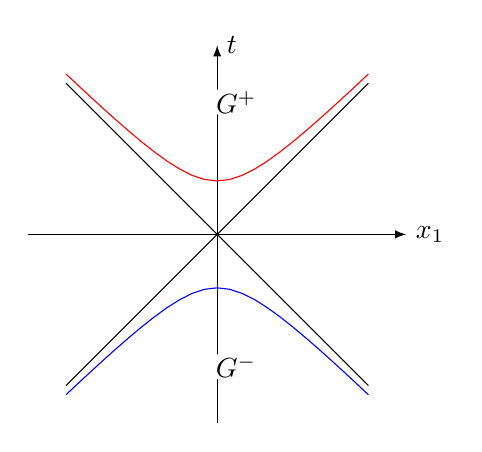
\begin{tikzpicture}[scale=0.48][>=latex]
				\coordinate (Origin)   at (0,0);
				\coordinate (XAxisMin) at (-5,0);
				\coordinate (XAxisMax) at (5,0);
				\coordinate (YAxisMin) at (0,-5);
				\coordinate (YAxisMax) at (0,5);
				\draw [thin,-latex] (XAxisMin) -- (XAxisMax) node[right] {$x_1$};% Draw x axis
				\draw [thin,-latex] (YAxisMin) -- (YAxisMax) node[right] {$t$};% Draw y axis
				%\draw [thin,-latex] (1.5,0.75) -- (-3,-1.5) node[left] {$x_2$};% Draw x axis
				
				%\clip (-5,-5) rectangle (10cm,10cm); % Clips the picture...
				
				\draw[thin] (0,0) -- (4,4);
				\draw[thin] (0,0) -- (-4,4);
				
				\onslide<1>{	\draw[red] plot[domain=-4:4] (\x,{sqrt(\x* \x+2)});
					\node[fill=white,rounded corners=1pt,inner sep=0.5pt] at (0.5,3.5) {$G^+$};}
			
				
				\draw[thin] (0,0) -- (4,-4);
				\draw[thin] (0,0) -- (-4,-4);
				\onslide<2>{\draw[blue] plot[domain=-4:4] (\x,{-sqrt(\x* \x+2)});
					\node[fill=white,rounded corners=1pt,inner sep=0.5pt] at (0.5,-3.5) {$G^-$};}
				
				
				
				
				
				
				
				\end{tikzpicture}
			\end{block}
			
		\end{column}
	
	\begin{column}{.48\linewidth}
		
		\only<1>{Un insieme di livello della soluzione fondamentale \textcolor{red}{\textbf{ritardata}} \[	G^{+}(t,\mf{x})=\frac{\Theta( t)}{2\pi}\frac{\Theta(t^2-|\mf{x}|^2)}{\sqrt{t^2-|\mf{x}|^2}}	\]
		$\supp\, G^+\subset$ cono luce \textcolor{red}{\textbf{futuro}}}
		\only<2>{Un insieme di livello della soluzione fondamentale \textcolor{red}{\textbf{avanzata}} \[	G^{-}(t,\mf{x})=\frac{\Theta(-t)}{2\pi}\frac{\Theta(t^2-|\mf{x}|^2)}{\sqrt{t^2-|\mf{x}|^2}}	\]	$\supp\, G^-\subset$ cono luce \textcolor{red}{\textbf{passato}}}
	\end{column}
	
	\end{columns}
	
	
	
	
	
	
\end{frame}

\begin{frame}
	\framesubtitle{Le soluzioni fondamentali in Minkowski}
	\frametitle{Il caso $n=3$ - onde nello spazio}
	
	\begin{columns}[t]
		\begin{column}{.48\linewidth}
			
			\begin{block}
				
			\only<1>{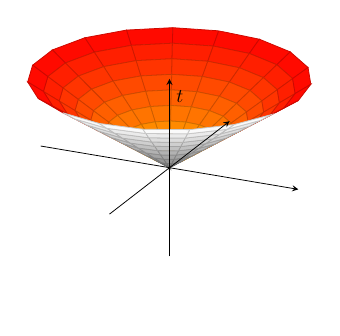
\begin{tikzpicture}[scale=0.7]
			\pgfplotsset{ticks=none}
			\begin{axis}[
			axis lines=center,
			axis on top,
			xlabel={}, ylabel={}, zlabel={$t$},
			domain=0:1,
			y domain=0:2*pi,
			%domain=-1:1,
			%y domain=-1:1,
			xmin=-1.5, xmax=1.5,
			ymin=-1.5, ymax=1.5, zmin=-1.0,
			%every axis x label/.style={at={(rel axis cs:0,0.5,0)},anchor=south},
			%every axis y label/.style={at={(rel axis cs:0.5,0,0)},anchor=north},
			every axis z label/.style={at={(rel axis cs:0.5,0.5,0.9)},anchor=west},
			mesh/interior colormap name=hot,
			colormap/blackwhite, 
			%samples=40,
			%samples y=60,
			samples=10,
			samples y=20,
			z buffer=sort,
			]
			\addplot3 [ surf, shader=faceted] ({(1.5*x*cos(deg(y))},{1.5*x*sin(deg(y))},{x});
			\addplot3 [opacity=0, fill opacity=0, surf, shader=faceted] ({(1.5*(-x)*cos(deg(y))},{1.5*(-x)*sin(deg(y))},{-x});
			
			
			\end{axis}
			\end{tikzpicture}}
	
		
		\only<2>{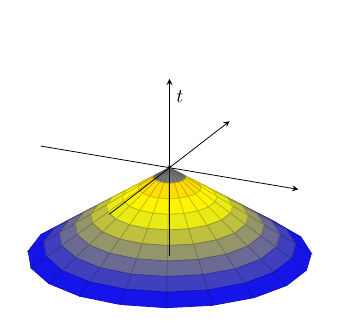
\begin{tikzpicture}[scale=0.7]
		\pgfplotsset{ticks=none}
		\begin{axis}[
		axis lines=center,
		axis on top,
		xlabel={}, ylabel={}, zlabel={$t$},
		domain=0:1,
		y domain=0:2*pi,
		%domain=-1:1,
		%y domain=-1:1,
		xmin=-1.5, xmax=1.5,
		ymin=-1.5, ymax=1.5, zmin=-1.0,
		%every axis x label/.style={at={(rel axis cs:0,0.5,0)},anchor=south},
		%every axis y label/.style={at={(rel axis cs:0.5,0,0)},anchor=north},
		every axis z label/.style={at={(rel axis cs:0.5,0.5,0.9)},anchor=west},
		mesh/interior colormap name=hot,
		colormap/blackwhite, 
		%samples=40,
		%samples y=60,
		samples=10,
		samples y=20,
		z buffer=sort,
		]
		\addplot3 [opacity=0, fill opacity=0, surf, shader=faceted] ({(1.5*x*cos(deg(y))},{1.5*x*sin(deg(y))},{x});
		\addplot3 [surf, shader=faceted] ({(1.5*(-x)*cos(deg(y))},{1.5*(-x)*sin(deg(y))},{-x});
			
			
			\end{axis}
			\end{tikzpicture}}
		
			\end{block}
			
		\end{column}
		
		\begin{column}{.48\linewidth}
			
			\only<1>{Il supporto della soluzione fondamentale \textcolor{red}{\textbf{ritardata}} \[	G^{+}(t,\mf{x})=\frac{\Theta( t)}{4\pi}\frac{\delta(t- |\mf{x}|)}{|\mf{x}|}	\]
				$\supp\, G^+$ � il \textcolor{red}{\textbf{bordo}} del cono luce \textcolor{red}{\textbf{futuro}}}
			\only<2>{Il supporto della soluzione fondamentale \textcolor{red}{\textbf{avanzata}} \[	G^{-}(t,\mf{x})=\frac{\Theta(-t)}{4\pi}\frac{\delta(t+ |\mf{x}|)}{|\mf{x}|}	\]
				$\supp\, G^-$ � il \textcolor{red}{\textbf{bordo}} del cono luce \textcolor{red}{\textbf{passato}}}
		\end{column}
		
	\end{columns}
	
	
	
	
	
	
\end{frame}


\begin{frame}
	
	\frametitle{Il Principio di Huygens}
		\framesubtitle{Le soluzioni fondamentali in Minkowski}
		
		\begin{columns}[t]
			
			\begin{column}{.48\linewidth}
				
				\begin{block}
					
					\only<1>{\includegraphics[width=\linewidth, scale=0.7]{geogebra-export}}
					\only<2>{\animategraphics[loop,controls,width=\linewidth]{12}{gif/giphy-}{0}{40}}
					\only<3>{\animategraphics[loop,controls,width=\linewidth]{12}{gif2/gif2-}{0}{49}}
				\end{block}
			\end{column}
			
			
			\begin{column}{.48\linewidth}
				
				Il supporto di $G^\pm$ coincide con il bordo del cono luce solo se $n>1$ � dispari.\\ \pause
				\bigskip
				 In 2D l'effetto dell'onda viene percepito \textcolor{red}{\textbf{anche dopo}} che il segnale � arrivato.\\ \pause
				\bigskip
				Le onde 3D si propagano solo sulla \textcolor{red}{\textbf{superficie sferica}} del fronte d'onda.
			
				
			\end{column}
			
			
			
			
		\end{columns}
		
		

		
	
\end{frame}


%\begin{block}

%In presenza di campo gravitazionale non nullo, dobbiamo ambientare le equazioni d'onda su variet� curve
%\end{block}\bigskip


\begin{frame}
	\frametitle{Lo spaziotempo come variet� differenziabile}
	%\framesubtitle{Le onde in un ambiente curvo}
	
	
	

		\begin{columns}
			\begin{column}{.60\linewidth}
				\only<1,2>{
			
			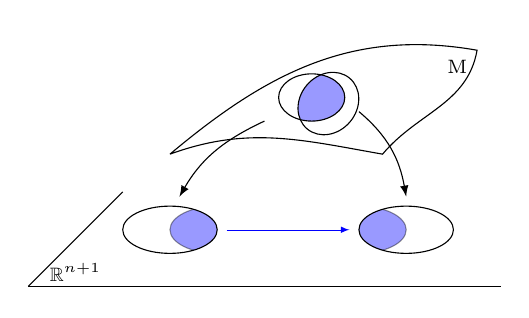
\begin{tikzpicture}[scale=0.6]
			\tikzstyle{every node}=[font=\scriptsize]
			\draw (0,0)  -- (10,0);
			\draw (0,0) -- (2,2);
			\node at (1,0.3) {$\mR^{n+1}$};
			
			\begin{scope}
			\clip (3,1.2) ellipse (1cm and 0.5cm);
			\draw [draw=black, fill=blue, opacity=0.4] (4,1.2) ellipse (1cm and 0.5cm);
			\end{scope}
			
			\begin{scope}
			\clip (8,1.2) ellipse (1cm and 0.5cm);
			\draw [draw=black, fill=blue, opacity=0.4] (7,1.2) ellipse (1cm and 0.5cm);
			\end{scope}
			
			\draw (3,1.2) ellipse (1cm and 0.5cm);
			%\node at (3,0.4) {$\varphi_i(U_i) $};
			
			
			\draw [-latex] (5,3.5) to[out=-155,in=60] (3.2,1.9) %node at (4,2.5) {$\varphi_i$}
			;
			
			
			\draw (8,1.2) ellipse (1cm and 0.5cm);
		%	\node at (8,0.4) {$\varphi_j(U_j) $};
			
			\draw [-latex] (7,3.7) to[out=-40,in=100] (8,1.9) %node at (8.2,2.5) {$\varphi_j$}
			;
			
			
			\draw [ultra thin,-latex, color=blue] (4.2, 1.2) -- (6.8,1.2) %node [pos=0.5,above] {$\varphi_i\circ\varphi_j^{-1}$}
			;
			\draw (3,2.8) to[out=40,in=170] (9.5,5) node[below left] {$\mathrm{M}$} to[out=-100,in=50]  (7.5,2.8) to[out=170,in=20] (3,2.8);
			
			%\node at (5.1,3.7) {$U_i$};
			%\node at (7.1,4.5) {$U_j$};
			
			
			\begin{scope}
			\clip (6,4) ellipse (0.7cm and 0.5cm);
			\fill[blue, opacity=0.4, rotate around={-40:(6.2,4)}] (6.4,4) ellipse (0.6cm and 0.7cm);
			\end{scope}
			\draw [thin] (6,4) ellipse (0.7cm and 0.5cm);
			\draw [thin, rotate around={-40:(6.2,4)}] (6.4,4) ellipse (0.6cm and 0.7cm);
			
			\end{tikzpicture}
					
			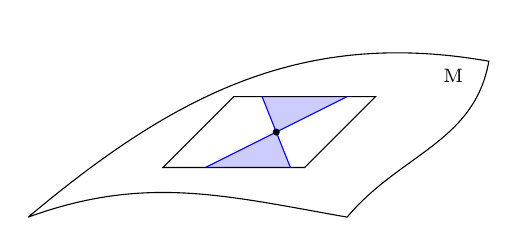
\begin{tikzpicture}[scale=0.9]
			\tikzstyle{every node}=[font=\scriptsize]
			
			\draw (1,2.8) to[out=40,in=170] (7.5,5) node at (7,4.8) {$\mathrm{M}$}
			to[out=-100,in=50]  (5.5,2.8) to[out=170,in=20] (1,2.8);
			
			\begin{scope}[shift={(0.5,0)},scale=1]
			\clip (2.2,3.4)-- (4.7,3.4) -- (5.7,4.6) -- (3.2,4.6) -- cycle;
			\draw [draw=black, thin, fill=white] (2.4,3.5)-- (4.4,3.5) -- (5.4,4.5) -- (3.4,4.5) -- cycle;
			%\draw [ultra thin, dashed] (1,2.8) to[out=40,in=170] (7.5,5) %node at (7,4.8) {$\mathrm{M}$}
			% to[out=-100,in=50]  (5.5,2.8) to[out=170,in=20] (1,2.8);
			
			\draw [thin, color=blue, fill=blue, fill opacity=0.2] (3,3.5) -- (4,4) -- (4.2,3.5) ;
			
			\draw [thin, color=blue, fill=blue, fill opacity=0.2] (3.8,4.5) -- (4,4) -- (5,4.5);
			
			%\draw [thin, color=blue, fill=blue, fill opacity=0.2] (3,3.5) -- (5,4.5)-- (3.8,4.5) -- (4.2,3.5) -- (3.8,4.5);
			\fill [black] (4,4) circle (0.05cm) %node [left] {$x$}
			;
			\end{scope}
			
			%\node at (5.3,4) {$\mathrm{T}_x\mathrm{M}$};
			
			\end{tikzpicture}}
			
			\only<3>{	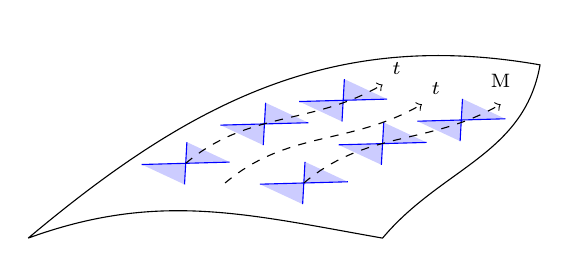
\begin{tikzpicture}[scale=1]
				\tikzstyle{every node}=[font=\scriptsize]
				
				\draw (1,2.8) to[out=40,in=170] (7.5,5) node at (7,4.8) {$\mathrm{M}$} to[out=-100,in=50]  (5.5,2.8) to[out=170,in=20] (1,2.8);
				
				
				\begin{scope}[shift={(-0.5,0.25)},scale=1]
				
				
				\begin{scope}[shift={(1.5,1.5)},scale=0.5, rotate around={-25:(4,4)}]
				\clip (2.2,3.4)-- (4.7,3.4) -- (5.7,4.6) -- (3.2,4.6) -- cycle;
				\draw [thin, color=blue, fill=blue, fill opacity=0.2] (3,3.5) -- (4,4) -- (4.2,3.5) ;
				\draw [thin, color=blue, fill=blue, fill opacity=0.2] (3.8,4.5) -- (4,4) -- (5,4.5);
				\begin{scope}[shift={(4,4)},scale=1]
			%	\draw [-latex, color=red] (-0.4,-0.4)-- (0.4,0.4);
				\end{scope}
				
				\end{scope}
				
				\begin{scope}[shift={(2.5,2)},scale=0.5, rotate around={-25:(4,4)}]
				\clip (2.2,3.4)-- (4.7,3.4) -- (5.7,4.6) -- (3.2,4.6) -- cycle;
				\draw [thin, color=blue, fill=blue, fill opacity=0.2] (3,3.5) -- (4,4) -- (4.2,3.5) ;
				\draw [thin, color=blue, fill=blue, fill opacity=0.2] (3.8,4.5) -- (4,4) -- (5,4.5);
				\begin{scope}[shift={(4,4)},scale=1]
			%	\draw [-latex, color=red] (-0.4,-0.4)-- (0.4,0.4);
				\end{scope}
				\end{scope}
				
				\begin{scope}[shift={(3.5,2.3)},scale=0.5, rotate around={-25:(4,4)}]
				\clip (2.2,3.4)-- (4.7,3.4) -- (5.7,4.6) -- (3.2,4.6) -- cycle;
				\draw [thin, color=blue, fill=blue, fill opacity=0.2] (3,3.5) -- (4,4) -- (4.2,3.5) ;
				\draw [thin, color=blue, fill=blue, fill opacity=0.2] (3.8,4.5) -- (4,4) -- (5,4.5);
				\begin{scope}[shift={(4,4)},scale=1]
			%	\draw [-latex, color=red] (-0.4,-0.4)-- (0.4,0.4);
				\end{scope}
				\end{scope}
				
				\draw [ ->, dashed, color=black] (3.5,3.5) to[out=40,in=-150] (6,4.5)node[above right] {$t$};
				\end{scope}
				
				\begin{scope}[shift={(1,0)},scale=1]
				
				
				\begin{scope}[shift={(1.5,1.5)},scale=0.5, rotate around={-25:(4,4)}]
				\clip (2.2,3.4)-- (4.7,3.4) -- (5.7,4.6) -- (3.2,4.6) -- cycle;
				\draw [thin, color=blue, fill=blue, fill opacity=0.2] (3,3.5) -- (4,4) -- (4.2,3.5) ;
				\draw [thin, color=blue, fill=blue, fill opacity=0.2] (3.8,4.5) -- (4,4) -- (5,4.5);
				\begin{scope}[shift={(4,4)},scale=1]
			%	\draw [-latex, color=red] (-0.4,-0.4)-- (0.4,0.4);
				\end{scope}
				
				\end{scope}
				
				\begin{scope}[shift={(2.5,2)},scale=0.5, rotate around={-25:(4,4)}]
				\clip (2.2,3.4)-- (4.7,3.4) -- (5.7,4.6) -- (3.2,4.6) -- cycle;
				\draw [thin, color=blue, fill=blue, fill opacity=0.2] (3,3.5) -- (4,4) -- (4.2,3.5) ;
				\draw [thin, color=blue, fill=blue, fill opacity=0.2] (3.8,4.5) -- (4,4) -- (5,4.5);
				\begin{scope}[shift={(4,4)},scale=1]
			%	\draw [-latex, color=red] (-0.4,-0.4)-- (0.4,0.4);
				\end{scope}
				\end{scope}
				
				\begin{scope}[shift={(3.5,2.3)},scale=0.5, rotate around={-25:(4,4)}]
				\clip (2.2,3.4)-- (4.7,3.4) -- (5.7,4.6) -- (3.2,4.6) -- cycle;
				\draw [thin, color=blue, fill=blue, fill opacity=0.2] (3,3.5) -- (4,4) -- (4.2,3.5) ;
				\draw [thin, color=blue, fill=blue, fill opacity=0.2] (3.8,4.5) -- (4,4) -- (5,4.5);
				\begin{scope}[shift={(4,4)},scale=1]
			%	\draw [-latex, color=red] (-0.4,-0.4)-- (0.4,0.4);
				\end{scope}
				\end{scope}
				
				\draw [ ->, dashed, color=black] (3.5,3.5) to[out=40,in=-150] (6,4.5);
				\end{scope}
				\draw [->, dashed, color=black] (3.5,3.5) to[out=40,in=-150] (6,4.5) node[above right] {$t$};
				%\node at (3.3,3.3) {$X$};
				
				\end{tikzpicture}}
			
			
			\end{column}
		
		\begin{column}{.40\linewidth}
			Una variet� differenziabile $\mM$ � \textcolor{red}{\textbf{localmente omeomorfa}} a $\mR^{n+1}$ e decorata con
			\medskip
				\begin{itemize}
					\item spazio tangente Minkowskiano\pause
					\item metrica $g$\pause
					\item orientazione temporale (\textcolor{red}{\textbf{spaziotempo}})
				\end{itemize}
		\end{column}
		
		\end{columns}

				
	
	
	
	
\end{frame}


\begin{frame}
	\frametitle{Spazitempi Globalmente Iperbolici}
	\begin{itemize}
		\item $\ds \mM\simeq\mR\times S\longrightarrow \{t\}\times S$ � \textcolor{red}{\textbf{ipersuperficie}} a tempo costante su cui porre dati iniziali \medskip
	\end{itemize}
	
	\begin{columns}
		\begin{column}{.48\linewidth}
			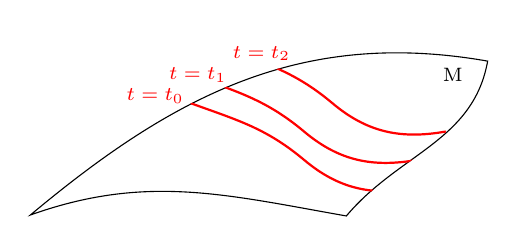
\begin{tikzpicture}[scale=0.9]
			\tikzstyle{every node}=[font=\scriptsize]
			
			\begin{scope}
			\clip[shift={(-0.5,0)}] (1,2.8) to[out=40,in=170] (7.5,5) to[out=-100,in=50]  (5.5,2.8) to[out=170,in=20] (1,2.8);
			\draw[shift={(-0.5,0)}, thick] (1,2.8) to[out=40,in=170] (7.5,5) node at (7,4.8) {$\mathrm{M}$} to[out=-100,in=50]  (5.5,2.8) to[out=170,in=20] (1,2.8);
			
			\draw[red,thick, scale=0.8, shift={(1.5,0.5)}] (2,5) to[out=-20,in=140] (4,4) to[out=-40,in=190] (6,3.5);
			\draw[red,thick, scale=0.8, shift={(1.5,1)}] (2,5) to[out=-20,in=140] (4,4) to[out=-40,in=190] (6,3.5);
			\draw[red,thick, scale=0.8, shift={(2,1.5)}] (2,5) to[out=-20,in=140] (4,4) to[out=-40,in=190] (6,3.5);
			
			
			\end{scope}
			\node at (2.3,4.5) {\textcolor{red}{${t=t_0}$}};
			\node at (2.9,4.8) {\textcolor{red}{${t=t_1}$}};
			\node at (3.8,5.1) {\textcolor{red}{${t=t_2}$}};
			
			
			
			
			
			\end{tikzpicture}
		\end{column}\pause
		\begin{column}{.48\linewidth}
			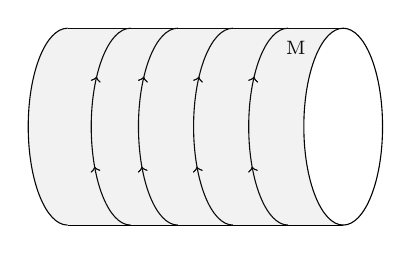
\begin{tikzpicture}
			\tikzstyle{every node}=[font=\scriptsize]
			\begin{scope}[rotate around={-90:(0,0)}]
			\draw (0,0) ellipse (1.25 and 0.5) ;
			\node at (-1,-0.6) {$\mM$};
			
			\draw (-1.25,0) -- (-1.25,-3.5);
			\draw (-1.25,-3.5) arc (180:360:1.25 and 0.5);
			
			\draw[->-,->>-] (-1.25,-2.1) arc (180:360:1.25 and 0.5);
			\draw[->-,->>-] (-1.25,-1.4) arc (180:360:1.25 and 0.5);
			\draw[->-,->>-] (-1.25,-0.7) arc (180:360:1.25 and 0.5);
			\draw[->-,->>-] (-1.25,-2.7) arc (180:360:1.25 and 0.5);
			
			%\draw[red,thick] (0,-4) -- (0,-0.5);
			%\draw [dashed] (-1.25,-3.5) arc (180:360:1.25 and -0.5);
			\draw (1.25,-3.5) -- (1.25,0);  
			\fill [gray,opacity=0.1] (-1.25,0) -- (-1.25,-3.5) arc (180:360:1.25 and 0.5) -- (1.25,0) arc (0:180:1.25 and -0.5);
			%\node[fill=white,rounded corners=1pt,inner sep=0.5pt] at (-0.2,-2) {\textcolor{red}{$t=t_0=t_1=\dots$}};
			\end{scope}
			
			\end{tikzpicture}
		\end{column}
	\end{columns}\medskip
	\begin{itemize}
		\item	Assenza di curve chiuse causali $\longrightarrow$ no \textcolor{red}{\textbf{paradossi temporali}}
	\end{itemize}
	

\end{frame}

\begin{frame}
	
	%	\frametitle{Lo spaziotempo come variet� differenziabile}
	\frametitle{Spazitempi di interesse fisico}
	
	\begin{itemize}
		\item Lo spaziotempo \textcolor{red}{\textbf{cosmologico}} $$\mM_c=\mR\times\mR^n$$ con metrica $$g_c= -\dd t^2 + f^2(t)\, \dd\mf{x}^2$$
		descrive un universo con fattore di espansione $f(t)$\bigskip%\pause
		
		\begin{columns}
			\begin{column}{.66\linewidth}
				\item Lo spaziotempo di \textcolor{red}{\textbf{Schwarzschild}} $$\mM_s=\mR\times(2m,+\infty)	\times \mathrm{S}^2$$ con metrica\\ $g_s=-\left(1-\frac{2m}{r}\right)\dd t^2+\left(1-\frac{2m}{r}\right)^{-1}\dd r^2	+r^2\dd\Omega^2$\\
				descrive l'esterno di un \textcolor{red}{\textbf{buco nero}} non rotante di massa $m$ e raggio $2m$
			\end{column}
			
			\begin{column}{.34\linewidth}
				\begin{block}
					\centering
					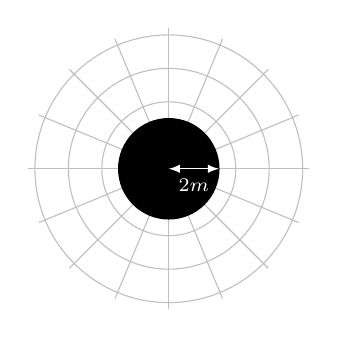
\begin{tikzpicture}[scale=0.425][>=latex]
					\tikzstyle{every node}=[font=\scriptsize]
					%\filldraw [fill=green!20!white, draw=green!50!black] (0:1) -- (0:2) arc[radius=2, start angle=0, end angle= 45] -- (45:1) arc[radius=1, start angle=45, end angle= 0] -- cycle;
					
					
					% Draw the lines at multiples of pi/12
					\foreach \ang in {0,...,15} {
						\draw [lightgray] (0,0) -- (\ang * 180 / 8:4.2);
					}
					
					% Concentric circles and radius labels
					\foreach \s in {0, 1, 2, 3, 4} {
						%\draw [lightgray] (0,0) circle (\s + 0.5);
						\draw[lightgray] (0,0) circle (\s);
						%\node [fill=white] at (\s, 0) [below] {\scriptsize $\s$};
					}
					\draw[black, fill=black] (0,0) circle (1.5);
					\draw[white, latex-latex] (0,0) -- (1.5,0) node[pos=0.5,below] {\textcolor{white}{$2m$}};
					
					
					
					\end{tikzpicture}
				\end{block}
				
			\end{column}
		\end{columns}
	\end{itemize}
	
	
		
		
		
	
\end{frame}


\begin{frame}
	
%	\frametitle{Lo spaziotempo come variet� differenziabile}
	\frametitle{Operatori d'onda in ambiente curvo}
		
	Gli operatori di tipo ondulatorio si generalizzano in base alla \textcolor{red}{\textbf{metrica}} locale $g$
	
	\begin{block}{Operatore generalizzato di d'Alembert}
		$$	P=-g^{ij}(x)\frac{\partial^2}{\partial x^i\partial x^j}+a^j(x)\parz{}{x^j}+b(x)$$
		
	\end{block}	\pause \bigskip

	In particolare l'operatore d'onda diventa
	\[	\Box=-\frac{1}{\sqrt{|g|}}\partial_i\left(\sqrt{|g|}g^{ij}\partial_j\right)			\]
	
	
\end{frame}

\begin{frame}
	\frametitle{Operatori d'onda in ambiente curvo}
	
	\begin{block}{\centering Spaziotempo cosmologico}
		$$\ds \Box =\frac{\partial^2}{\partial t^2}-\frac{3}{f(t)}\frac{\partial}{\partial t}+\frac{1}{f^2(t)}\Delta$$
	\end{block}\medskip
	\begin{block}{\centering Spaziotempo di Schwarzschild}
		$\ds \Box=	\left(1-\frac{2m}{r}\right)^{-1}\frac{\partial^2}{\partial t^2}-\left(1-\frac{2m}{r}\right)\frac{1}{r^2}\frac{\partial}{\partial r}(r^2-2mr)\frac{\partial}{\partial r}+\frac{1}{r^2}\Delta_{\theta,\varphi}$
	\end{block}\medskip
	
	Cade la simmetria traslazionale. La soluzione fondamentale \[	Pu_x=\delta_x		\] deve essere cercata \textcolor{red}{\textbf{punto per punto}} senza poter usare Fourier
	
\end{frame}

\begin{frame}
	\frametitle{Le distribuzioni di Riesz}
	Ritroviamo le soluzioni fondamentali su Minkowski sfruttando le \textcolor{red}{\textbf{distribuzioni di Riesz}}, definite per $\alpha\in\mC$ a partire dalla formula \bigskip
	\begin{block}
		
		\begin{equation*}
		R_\pm(\alpha)(x):=
		\frac{2^{1-\alpha}\pi^{\frac{1-n}{n+1}}}{\Gamma(\frac\alpha{2})\Gamma(\frac{\alpha-n+1}{2})}\left(-\langle x,x\rangle\right)^{\frac{\alpha-n-1}{2}}
		\end{equation*}
	\centering	se $x$ � nel cono luce futuro $(+)$/passato $(-)$ e $0$ altrimenti, con $\Re\alpha>n+1$
	\end{block}\pause\bigskip
	
	\begin{columns}
		\begin{column}{.20\linewidth}
			\begin{block}
				
				$\ds \Box R_\pm(2)=\delta_0$
			\end{block}
		\end{column}
	
		\begin{column}{.78\linewidth}
		\centering $R_\pm(2)$ sono le soluzioni fondamentali \textcolor{red}{\textbf{ritardata}} $(+)$ e \textcolor{red}{\textbf{avanzata}} $(-)$
	\end{column}
	
	\end{columns}
	
	 
	
	
	
\end{frame}


\begin{frame}
	\frametitle{La soluzione fondamentale locale}
	Le distribuzioni di Riesz si estendono localmente dal tangente Minkowskiano al curvo.\\ \bigskip
	\centering
			\begin{tikzpicture}[scale=1.3]
			\tikzstyle{every node}=[font=\scriptsize]
			
			\draw[shift={(-0.5,0)}] (1,2.8) to[out=40,in=170] (7.5,5) node at (7,4.8) {$\mathrm{M}$} to[out=-100,in=50]  (5.5,2.8) to[out=170,in=20] (1,2.8);
			
			\begin{scope}[shift={(0,2)},scale=1]
			\clip (2.2,3.4)-- (4.7,3.4) -- (5.7,4.6) -- (3.2,4.6) -- cycle;
			\draw [draw=black, thin, fill=white] (2.4,3.5)-- (4.4,3.5) -- (5.4,4.5) -- (3.4,4.5) -- cycle;
			%\draw [ultra thin, dashed] (1,2.8) to[out=40,in=170] (7.5,5) %node at (7,4.8) {$\mathrm{M}$}
			% to[out=-100,in=50]  (5.5,2.8) to[out=170,in=20] (1,2.8);
			
			\visible<2>{\draw [thin, color=blue, fill=blue, fill opacity=0.2] (3,3.5) -- (4,4) -- (4.2,3.5) ;}
			
			\visible<1>{\draw [thin, color=blue, fill=blue, fill opacity=0.2] (3.8,4.5) -- (4,4) -- (5,4.5);}
			
			%\draw [thin, color=blue, fill=blue, fill opacity=0.2] (3,3.5) -- (5,4.5)-- (3.8,4.5) -- (4.2,3.5) -- (3.8,4.5);
			\only<1>{\fill [black] (4,4) circle (0.05cm) node [left] {$R_+(\alpha)$};}
			\only<2>{\fill [black] (4,4) circle (0.05cm) node [above] {$R_-(\alpha)$};}
			
			\end{scope}
			
			
			
			
			\draw [ dashed] (4,6) -- (4,5.5);
			\draw [ -latex] (4,5.5) -- (4,4) %node [pos=0.4, right] {$\exp_p$}
			;
			\node at (5.3,4) {$\Omega$};
			\only<1>{\node at (3,3.5) {$R_+^\Omega(\alpha,x)$};}
			\only<2>{\node at (3,3.5) {$R_-^\Omega(\alpha,x)$};}
			
			
			\begin{scope}[shift={(3.25,4)},scale=0.6]
			\clip plot [smooth cycle] coordinates { (0,0) (1,1) (3,0) (1.5,-1)};
			\draw [black, thick] plot [smooth cycle] coordinates { (0,0) (1,1) (3,0) (1.5,-1)};
			
			\begin{scope}[shift={(-3.55,-4.8)},scale=1.2]
			
			\visible<2>{\draw [thin, color=blue, fill=blue, fill opacity=0.2] (3,3.5) -- (4,4) -- (4.6,2.5) ;}
			
			\visible<1>{\draw [thin, color=blue, fill=blue, fill opacity=0.2] (3.4,5.5) -- (4,4) -- (5,4.5);}
			
			%\draw [thin, color=blue, fill=blue, fill opacity=0.2] (3,3.5) -- (5,4.5)-- (3.8,4.5) -- (4.2,3.5) -- (3.8,4.5);
			\fill [black] (4,4) circle (0.05cm) node [left] {$x$}
			;
			
			\end{scope}
			
			\end{scope}
			
			
			\end{tikzpicture}
	
	
\end{frame}



	\begin{frame}
	\frametitle{Il problema ai dati iniziali locale}
	
	Con le soluzioni fondamentali trovate risolviamo il problema di Cauchy localmente
	
	\begin{columns}
	\begin{column}{.60\linewidth}
	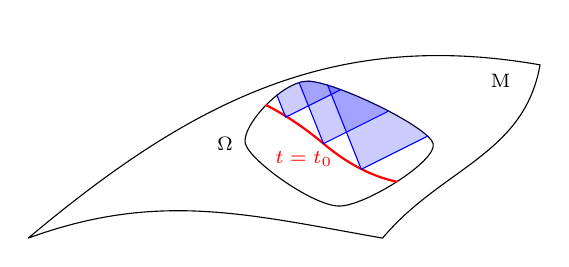
\begin{tikzpicture}[scale=1]
	\tikzstyle{every node}=[font=\scriptsize]
	
	\draw[shift={(-0.5,0)}] (1,2.8) to[out=40,in=170] (7.5,5) node at (7,4.8) {$\mathrm{M}$} to[out=-100,in=50]  (5.5,2.8) to[out=170,in=20] (1,2.8);
	\node at (3,4) {$\Omega$};
	\node at (4,3.8) {\textcolor{red}{${t=t_0}$}};
	%\node at (3,3.5) {$R_+^\Omega(\alpha,x)$};
	
	
	
	\begin{scope}[shift={(3.25,4)},scale=0.8]
	\clip plot [smooth cycle] coordinates { (0,0) (1,1) (3,0) (1.5,-1)};
	\draw [black, thick] plot [smooth cycle] coordinates { (0,0) (1,1) (3,0) (1.5,-1)};
	
	\begin{scope}[shift={(-3.55,-4.8)},scale=1.2]
	\draw[red,thick] (2,5) to[out=-20,in=140] (4,4) to[out=-40,in=190] (6,3.5);
	
	\draw [thin, color=blue, fill=blue, fill opacity=0.2] (3.4,5.5) -- (4,4) -- (5,4.5);
	\begin{scope}[shift={(-0.5,0.35)},scale=1]
	\draw [thin, color=blue, fill=blue, fill opacity=0.2] (3.4,5.5) -- (4,4) -- (5,4.5);
	\end{scope}
	\begin{scope}[shift={(0.5,-0.34)},scale=1]
	\draw [thin, color=blue, fill=blue, fill opacity=0.2] (3.4,5.5) -- (4,4) -- (5,4.5);
	\end{scope}
	
	%\draw [thin, color=blue, fill=blue, fill opacity=0.2] (3,3.5) -- (5,4.5)-- (3.8,4.5) -- (4.2,3.5) -- (3.8,4.5);
	%\fill [black] (4,4) circle (0.05cm) node [left] {$x$}
	;
	
	\end{scope}
	
	\end{scope}
	
	
	\end{tikzpicture}
	\end{column}
	
	\begin{column}{.40\linewidth}
	
	\begin{block}{Problema ai dati iniziali}
	\begin{equation*}
	\begin{cases}
	P \psi=f\\
	\\
	\psi(t_0,\cdot)=\psi^0\\
	\\
	\parz{}{t}\psi(t_0,\cdot)=\psi^1.
	\end{cases}
	\end{equation*}
	\end{block}
	\end{column}
	
	
	\end{columns}\medskip
	
	
	\end{frame}

\begin{frame}
	\frametitle{Il problema ai dati iniziali globale}
	 Se lo spaziotempo � globalmente iperbolico, si ottengono soluzioni fondamentali \textcolor{red}{\textbf{globali}} $G^\pm$\medskip
	
	\begin{columns}
		\begin{column}{.43\linewidth}
			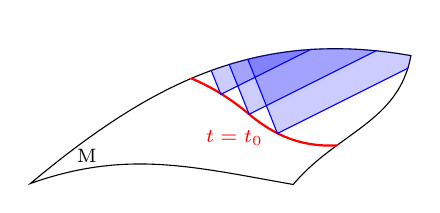
\begin{tikzpicture}[scale=0.75]
			\tikzstyle{every node}=[font=\scriptsize]
			
			
			\begin{scope}
			\clip[shift={(-0.5,0)}] (1,2.8) to[out=40,in=170] (7.5,5) to[out=-100,in=50]  (5.5,2.8) to[out=170,in=20] (1,2.8);
			\draw[shift={(-0.5,0)}, thick] (1,2.8) to[out=40,in=170] (7.5,5)  to[out=-100,in=50]  (5.5,2.8) to[out=170,in=20] (1,2.8);
			\node at (1.5,3.3) {$\mathrm{M}$};
			
			\begin{scope}[shift={(3.25,4)},scale=0.8]
			%\clip plot [smooth cycle] coordinates { (0,0) (1,1) (3,0) (1.5,-1)};
			%\draw [black, thick] plot [smooth cycle] coordinates { (0,0) (1,1) (3,0) (1.5,-1)};
			
			\begin{scope}[shift={(-3.55,-4.8)},scale=1.2]
			\draw[red,thick] (2,5) to[out=-20,in=140] (4,4) to[out=-40,in=190] (6,3.5);
			
			\draw [thin, color=blue, fill=blue, fill opacity=0.2] (3.4,5.5) -- (4,4) -- (7,5.5);
			\begin{scope}[shift={(-0.5,0.35)},scale=1]
			\draw [thin, color=blue, fill=blue, fill opacity=0.2] (3.4,5.5) -- (4,4) -- (7,5.5);
			\end{scope}
			\begin{scope}[shift={(0.5,-0.34)},scale=1]
			\draw [thin, color=blue, fill=blue, fill opacity=0.2] (3.4,5.5) -- (4,4) -- (7,5.5);
			\end{scope}
			
			%\draw [thin, color=blue, fill=blue, fill opacity=0.2] (3,3.5) -- (5,4.5)-- (3.8,4.5) -- (4.2,3.5) -- (3.8,4.5);
			%\fill [black] (4,4) circle (0.05cm) node [left] {$x$}
			;
			
			\end{scope}
			
			\end{scope}
			\end{scope}
			
			\node at (4,3.6) {\textcolor{red}{${t=t_0}$}};
			%\node at (3,3.5) {$R_+^\Omega(\alpha,x)$};
			
			
			
			
			
			
			\end{tikzpicture}
		\end{column}
		\begin{column}{.55\linewidth}
			\begin{block}
				
				\begin{itemize}
					\item la soluzione $\psi$ � unica e liscia
					\item supporto nel futuro causale e nel passato causale
				\end{itemize}
			\end{block}
			
		\end{column}
	\end{columns}

	
	
	
		
	
\end{frame}

\begin{frame}
	\frametitle{Conclusioni}
	Risultati ottenuti:
	\begin{itemize}
		\item<+-| alert@+> Costruzione delle soluzioni fondamentali per $\Box$ in Minkowski attraverso
		\begin{itemize}
			\item trasformata di Fourier
			\item distribuzioni di Riesz
		\end{itemize}
	
		\item<+-| alert@+> Estensione locale e globale delle soluzioni fondamentali su spazitempi globalmente iperbolici
	\end{itemize}
	Possibili sviluppi:
		\begin{itemize}
		\item<+-| alert@+> Estensione ad altri operatori (Dirac)
	\end{itemize}
	
\end{frame}
	
\end{document}